\documentclass[a4paper,12pt,twoside,final,toc=listof, bibliography=totoc, open=any]{scrbook}
\usepackage[usenames,dvipsnames]{xcolor} % Required for specifying custom colors and referring to colors by name
\usepackage{graphicx}
\usepackage[english]{babel}
\usepackage[latin1]{inputenc}
\usepackage{amsmath, amsthm,amssymb}
\usepackage{epstopdf}
\usepackage[authoryear, round]{natbib}
\usepackage[babel,english=american]{csquotes}
\usepackage[headsepline, automark]{scrpage2}
\usepackage[format=plain,indention=.5cm,margin=10pt,font=small,font=sf, labelfont=bf]{caption}
\usepackage{listings}
\usepackage{subcaption}
\usepackage{colortbl}
\usepackage{enumitem}
\usepackage{lipsum}
\usepackage[colorlinks, linkcolor=Aquamarine, citecolor=Aquamarine, urlcolor=black]{hyperref}
\usepackage[toc, index]{glossaries}
\usepackage{etoolbox}
\AtBeginEnvironment{description}{\pretocmd{\item}{\phantomsection}{}{\errmessage{couldn't patch item}}}

% modify tree style to make target bold

\makeglossaries

% make hyperlinks of glossary entries black
\renewcommand*{\glstextformat}[1]{\textcolor{black}{#1}}
% label glossaries with glo:<glossary-name>
\renewcommand*{\glsautoprefix}{glo:} 
\renewcommand{\glsseeitemformat}[1]{\glssymbol{#1}}



\definecolor{DarkGreen}{rgb}{0.0,0.4,0.0} % Comment color
\definecolor{highlight}{RGB}{255,251,204} % Code highlight color
\interfootnotelinepenalty 10000

\lstdefinestyle{defaultstyle}{ % Define a style for your code snippet, multiple definitions can be made if, for example, you wish to insert multiple code snippets using different programming languages into one document
language=Python, % Detects keywords, comments, strings, functions, etc for the language specified
backgroundcolor=\color[gray]{0.9}, % Set the background color for the snippet - useful for highlighting
basicstyle=\footnotesize\ttfamily, % The default font size and style of the code
breakatwhitespace=false, % If true, only allows line breaks at white space
breaklines=true, % Automatic line breaking (prevents code from protruding outside the box)
captionpos=t, % Sets the caption position: b for bottom; t for top
commentstyle=\color{gray}, % Style of comments within the code - dark green courier font
deletekeywords={}, % If you want to delete any keywords from the current language separate them by commas
%escapeinside={\%}, % This allows you to escape to LaTeX using the character in the bracket
firstnumber=1, % Line numbers begin at line 1
frame=single, % Frame around the code box, value can be: none, leftline, topline, bottomline, lines, single, shadowbox
frameround=tttt, % Rounds the corners of the frame for the top left, top right, bottom left and bottom right positions
keywordstyle=\color{blue}\bf, % Functions are bold and blue
morekeywords={}, % Add any functions no included by default here separated by commas
numbers=left, % Location of line numbers, can take the values of: none, left, right
numbersep=10pt, % Distance of line numbers from the code box
numberstyle=\tiny\color{gray}, % Style used for line numbers
rulecolor=\color{black}, % Frame border color
showstringspaces=false, % Don't put marks in string spaces
showtabs=false, % Display tabs in the code as lines
stepnumber=5, % The step distance between line numbers, i.e. how often will lines be numbered
stringstyle=\color{purple}, % Strings are purple
tabsize=2, % Number of spaces per tab in the code
}
\lstdefinestyle{smallstyle}{
style=defaultstyle,
basicstyle=\scriptsize\ttfamily, % The default font size and style of the code
}
\lstset{style=defaultstyle}
% Create a command to cleanly insert a snippet with the style above anywhere in the document
\newcommand{\insertcode}[3][\empty]{
	\ifthenelse{\equal{#1}{\empty}}
		{\begin{itemize}\item[]\lstinputlisting[caption=#3,label=#2,style=smallstyle]{#2}\end{itemize}} % The first argument is the script location/filename and the second is a caption for the 
		{\begin{itemize}\item[]\lstinputlisting[caption=#3,label=#1,style=smallstyle]{#2}\end{itemize}}}
\newglossaryentry{figtitlesize}{name=figtitlesize, type=index, description=\nopostdesc}
\newglossaryentry{xlim}{name=xlim, type=index, description=\nopostdesc}
\newglossaryentry{color}{name=color, type=index, description=\nopostdesc}
\newglossaryentry{meridionals}{name=meridionals, type=index, description=\nopostdesc}
\newglossaryentry{lsm}{name=lsm, type=index, description=\nopostdesc}
\newglossaryentry{land_color}{name=land\_color, type=index, description=\nopostdesc}
\newglossaryentry{maskless}{name=maskless, type=index, description=\nopostdesc}
\newglossaryentry{ticksize}{name=ticksize, type=index, description=\nopostdesc}
\newglossaryentry{linewidth}{name=linewidth, type=index, description=\nopostdesc}
\newglossaryentry{labelsize}{name=labelsize, type=index, description=\nopostdesc}
\newglossaryentry{ylim}{name=ylim, type=index, description=\nopostdesc}
\newglossaryentry{xticklabels}{name=xticklabels, type=index, description=\nopostdesc}
\newglossaryentry{latlon}{name=latlon, type=index, description=\nopostdesc}
\newglossaryentry{xticks}{name=xticks, type=index, description=\nopostdesc}
\newglossaryentry{figtitleweight}{name=figtitleweight, type=index, description=\nopostdesc}
\newglossaryentry{scale}{name=scale, type=index, description=\nopostdesc}
\newglossaryentry{arrowstyle}{name=arrowstyle, type=index, description=\nopostdesc}
\newglossaryentry{titleweight}{name=titleweight, type=index, description=\nopostdesc}
\newglossaryentry{maskgreater}{name=maskgreater, type=index, description=\nopostdesc}
\newglossaryentry{lonlatbox}{name=lonlatbox, type=index, description=\nopostdesc}
\newglossaryentry{labelweight}{name=labelweight, type=index, description=\nopostdesc}
\newglossaryentry{ticks}{name=ticks, type=index, description=\nopostdesc}
\newglossaryentry{ticklabels}{name=ticklabels, type=index, description=\nopostdesc}
\newglossaryentry{density}{name=density, type=index, description=\nopostdesc}
\newglossaryentry{streamplot}{name=streamplot, type=index, description=\nopostdesc}
\newglossaryentry{merilabelpos}{name=merilabelpos, type=index, description=\nopostdesc}
\newglossaryentry{tickweight}{name=tickweight, type=index, description=\nopostdesc}
\newglossaryentry{maskbetween}{name=maskbetween, type=index, description=\nopostdesc}
\newglossaryentry{maskgeq}{name=maskgeq, type=index, description=\nopostdesc}
\newglossaryentry{text}{name=text, type=index, description=\nopostdesc}
\newglossaryentry{xlabel}{name=xlabel, type=index, description=\nopostdesc}
\newglossaryentry{clabel}{name=clabel, type=index, description=\nopostdesc}
\newglossaryentry{proj}{name=proj, type=index, description=\nopostdesc}
\newglossaryentry{tight}{name=tight, type=index, description=\nopostdesc}
\newglossaryentry{enable}{name=enable, type=index, description=\nopostdesc}
\newglossaryentry{titlesize}{name=titlesize, type=index, description=\nopostdesc}
\newglossaryentry{parallels}{name=parallels, type=index, description=\nopostdesc}
\newglossaryentry{extend}{name=extend, type=index, description=\nopostdesc}
\newglossaryentry{yrotation}{name=yrotation, type=index, description=\nopostdesc}
\newglossaryentry{title}{name=title, type=index, description=\nopostdesc}
\newglossaryentry{ylabel}{name=ylabel, type=index, description=\nopostdesc}
\newglossaryentry{paralabelpos}{name=paralabelpos, type=index, description=\nopostdesc}
\newglossaryentry{rasterized}{name=rasterized, type=index, description=\nopostdesc}
\newglossaryentry{grid}{name=grid, type=index, description=\nopostdesc}
\newglossaryentry{axiscolor}{name=axiscolor, type=index, description=\nopostdesc}
\newglossaryentry{windplot}{name=windplot, type=index, description=\nopostdesc}
\newglossaryentry{xrotation}{name=xrotation, type=index, description=\nopostdesc}
\newglossaryentry{ocean_color}{name=ocean\_color, type=index, description=\nopostdesc}
\newglossaryentry{lineshapes}{name=lineshapes, type=index, description=\nopostdesc}
\newglossaryentry{yticklabels}{name=yticklabels, type=index, description=\nopostdesc}
\newglossaryentry{plotcbar}{name=plotcbar, type=index, description=\nopostdesc}
\newglossaryentry{countries}{name=countries, type=index, description=\nopostdesc}
\newglossaryentry{lengthscale}{name=lengthscale, type=index, description=\nopostdesc}
\newglossaryentry{ctickweight}{name=ctickweight, type=index, description=\nopostdesc}
\newglossaryentry{mask}{name=mask, type=index, description=\nopostdesc}
\newglossaryentry{bounds}{name=bounds, type=index, description=\nopostdesc}
\newglossaryentry{fontweight}{name=fontweight, type=index, description=\nopostdesc}
\newglossaryentry{cticksize}{name=cticksize, type=index, description=\nopostdesc}
\newglossaryentry{cmap}{name=cmap, type=index, description=\nopostdesc}
\newglossaryentry{figtitle}{name=figtitle, type=index, description=\nopostdesc}
\newglossaryentry{yticks}{name=yticks, type=index, description=\nopostdesc}
\newglossaryentry{reduceabove}{name=reduceabove, type=index, description=\nopostdesc}
\newglossaryentry{fontsize}{name=fontsize, type=index, description=\nopostdesc}
\newglossaryentry{arrowsize}{name=arrowsize, type=index, description=\nopostdesc}
\newglossaryentry{maskleq}{name=maskleq, type=index, description=\nopostdesc}
\newglossaryentry{legend}{name=legend, type=index, description=\nopostdesc}

% MapBase
\newglossaryentry{MapBase}{name=MapBase, description={Basic class that reads data from a NetCDF file and plots visualizes it on one axes}, type=main, text=\lstinline|MapBase|, symbol=\lstinline|nc2map.mapos.MapBase|}
\newglossaryentry{FieldPlot}{name=FieldPlot, description={Class that plots a two-dimensional field (e.g. temperature) and optionally overlained by a wind field}, type=main, text=\lstinline|FieldPlot|, parent=MapBase, symbol=\lstinline|nc2map.mapos.FieldPlot|}
\newglossaryentry{FieldPlot.data}{name=data, description={\gls{DataField} instance storing the data of the variable}, text=\lstinline|data|, symbol=\lstinline|FieldPlot.data|, parent=FieldPlot}
\newglossaryentry{WindPlot}{name=WindPlot, description={Class that plots a wind field (stream plot or quiver plot)}, type=main, text=\lstinline|WindPlot|, parent=MapBase, symbol=\lstinline|nc2map.mapos.WindPlot|}
\newglossaryentry{MapBase.meta}{name=meta, description={meta data property of the \gls{MapBase} instance which gives a dictionary containing all the meta data information of the specific variable}, symbol=\lstinline|MapBase.meta|, text=\lstinline|MapBase.meta|, symbol=\lstinline|MapBase.meta|, parent=MapBase}
\newglossaryentry{LinePlot}{name=LinePlot, description={Class to visualize one dimensional data in the NetCDF file}, text=\lstinline|LinePlot|, symbol=\lstinline|nc2map.mapos.LinePlot|}
\newglossaryentry{ViolinPlot}{name=ViolinPlot, description={Class to make a violin plot using the python \lstinline|seaborn.violinplot| function. Note that if you want to create an \lstinline|ViolinPlot| instance manually, this class (different from \gls{LinePlot} and \gls{MapBase} instances) does not extract the data from a \gls{reader}. Instead you have to pass it in manually at the initialization}, text=\lstinline|ViolinPlot|, symbol=\lstinline|nc2map.mapos.ViolinPlot|, see=ViolinEvaluator}
\newglossaryentry{MapBase.get_data}{name=MapBase.get\_data, description={Method of \gls{MapBase} (and \gls{LinePlot}) instances to extract the data from the reader}, parent=MapBase, see=reader.get_data, symbol=\lstinline|nc2map.mapos.MapBase.get_data|, text=\lstinline|get_data|}

% nc2map
\newglossaryentry{nc2map}{name=nc2map, description={Interactive python module to visualize NetCDF files on a map}, type=main, text=\lstinline|nc2map|}
\newglossaryentry{nc2map.load}{name=load, description={Function that loads \lstinline|pickle| files generated by the \gls{Maps.save} method and opens the \gls{Maps} instance with the previously saved settings}, text=\lstinline|load|, symbol={\lstinline|nc2map.load|}, parent=nc2map, see={Maps.save}}

\newglossaryentry{shp_utils}{name={shp\_utils}, description={Shape file module of the \gls{nc2map} module}, text=\lstinline|shp_utils|, symbol={\lstinline|nc2map.shp_utils|}}

% MapsManager
\newglossaryentry{MapsManager}{name=MapsManager, description={Basic class that controls multiple \gls{MapBase} instances}, type=main, text=\lstinline|MapsManager|, symbol=\lstinline|nc2map.MapsManager|}
\newglossaryentry{Maps}{name=Maps, description={Basic class for plotting in \gls{nc2map}. Controls multiple \gls{MapBase} instances}, type=main, text=\lstinline|Maps|, parent=MapsManager, symbol=\lstinline|nc2map.Maps|}
\newglossaryentry{Maps.update}{name=update, description={Update method of the \gls{Maps} class. Updates the chosen \gls{MapBase} instances by the given formatoptions. \gls{MapBase} instances may be chosen via \glspl{dimsidentifier}}, type=main, text=\lstinline|update|, parent=Maps, symbol={\lstinline|Maps.update|}}
\newglossaryentry{Maps.output}{name=output, description={Output method of the \gls{Maps} class. Exports the chosen \gls{MapBase} instances (or figures) into different (static) formats. \gls{MapBase} instances may be chosen via \glspl{dimsidentifier}}, type=main, text=\lstinline|output|, parent=Maps, symbol={\lstinline|Maps.output|}, see={Maps.make_movie}}
\newglossaryentry{Maps.make_movie}{name={make\_movie}, description={Movie method of the \gls{Maps} class. Exports the chosen \gls{MapBase} instances (or figures) into a movie of the specified format for the user given (or all) time steps. \gls{MapBase} instances may be chosen via \glspl{dimsidentifier}}, type=main, text=\lstinline|make_movie|, parent=Maps, symbol={\lstinline|Maps.make_movie|}, see={Maps.output}}
\newglossaryentry{MapsManager.addmap}{name={addmap}, description={Add a new MapBase instance to the \gls{MapsManager} instance. This function is used at the initialization of a \gls{Maps} instance.}, parent=MapsManager, text=\lstinline|addmap|, symbol=\lstinline|MapsManager.addmap|}
\newglossaryentry{MapsManager.addline}{name={addline}, description={Add a new LinePlot instance to the \gls{MapsManager} instance. This function is used at the initialization of a \gls{Maps} instance if \lstinline|linesonly=True| is set.}, parent=MapsManager, text=\lstinline|addline|, symbol=\lstinline|MapsManager.addline|}
\newglossaryentry{MapsManager.get_label_dict}{name={get\_label\_dict}, description={Helper function. Returns the meta data of the given \gls{MapBase} instance}, text=\lstinline|get_label_dict|, parent=MapsManager, symbol={\lstinline|Maps.get_label_dict|}, see={MapsManager.meta,MapBase.meta}}
\newglossaryentry{MapsManager.meta}{name={meta}, description={Property that returns a dictionary containing all the meta information in the \gls{MapBase} and \gls{LinePlot} instances of the \gls{MapsManager} instance}, parent=MapsManager, text=\lstinline|MapsManager.meta| see={MapsManager.get_label_dict,MapBase.meta}}
\newglossaryentry{MapsManager.get_maps}{name={get\_maps}, description={Helper function. Returns the \gls{MapBase} corresponding to the given \gls{dimsidentifier}}, text=\lstinline|get_maps|, parent=MapsManager, symbol={\lstinline|MapsManager.get_maps|}}
\newglossaryentry{Maps.save}{name=save, description={Helper function of the \gls{Maps} class. This method creates a \lstinline|pickle| file that can be loaded with the \gls{nc2map.load} function, to reinitialize of \gls{Maps} instance with all coordinated \gls{MapBase} instances and their settings}, text=\lstinline|save|, parent=Maps, symbol=\lstinline|Maps.save|, see={nc2map.load}}
\newglossaryentry{Maps.evaluate}{name=evaluate, description={Evaluator method that passes \gls{MapBase} instances to evaluators}, text=\lstinline|evaluate|, symbol=\lstinline|nc2map.Maps.evaluate|, parent=Maps, see={FldMeanEvaluator,ViolinEvaluator}}
\newglossaryentry{Maps.nextt}{name=nextt, description={Updates all MapBase instances controlled by the \gls{Maps} instances to the next time step}, parent=Maps, symbol=\lstinline|Maps.nextt|, see={Maps.prevt}, text=\lstinline|nextt|}
\newglossaryentry{Maps.prevt}{name=prevt, description={Updates all MapBase instances controlled by the \gls{Maps} instances to the next time step}, parent=Maps, symbol=\lstinline|Maps.prevt|, see={Maps.nextt}, text=\lstinline|prevt|}



\newglossaryentry{dimsidentifier}{name={Dimension identifiers}, description=\nopostdesc, type=main, plural={dimension identifiers}, text={dimension identifier}}
\newglossaryentry{var}{name=var, text={\lstinline|var|}, description={(plural: \texttt{vlst}). Identifier for the variable}, type=main, plural={\lstinline|vlst|}, parent=dimsidentifier}
\newglossaryentry{time}{name=time, text={\lstinline|time|}, description={Identifier for the time (as integer)}, type=main, parent=dimsidentifier}
\newglossaryentry{level}{name=level,text={\lstinline|level|}, description={Identifier for the vertical level (as integer)}, type=main, parent=dimsidentifier}
\newglossaryentry{name}{name=name, text={\lstinline|name|}, description={Identifier for the name of the \gls{MapBase} instance}, type=main, parent=dimsidentifier}

\newglossaryentry{fmt}{name=formatoption, symbol={\lstinline|fmt|}, description={Formatoption keywords that control the appearance of the plot (see \autoref{ch:fmt} for details).}}
\newglossaryentry{show_fmtkeys}{name={show\_fmtkeys}, description={Helper function to display the possible \gls{fmt} keywords}, symbol={\lstinline|nc2map.show_fmtkeys|}, text={\lstinline|show_fmtkeys|}, parent=fmt, see=get_fmtkeys}
\newglossaryentry{get_fmtkeys}{name={get\_fmtkeys}, description={Same as \gls{show_fmtkeys}, but returns a string.}, symbol={\lstinline|nc2map.get_fmtkeys|}, text={\lstinline|get_fmtkeys|}, parent=fmt, see=show_fmtkeys}
\newglossaryentry{show_fmtdocs}{name={show\_fmtdocs}, description={Helper function to display the possible \gls{fmt} keywords and their documentation}, symbol={\lstinline|nc2map.show_fmtdocs|}, text={\lstinline|show_fmtdocs|}, parent=fmt, see=get_fmtdocs}
\newglossaryentry{get_fmtdocs}{name={get\_fmtdocs}, description={Same as \gls{show_fmtdocs}, but instead of displaying the documentation, returns a dictionary with formatoption keywords as keys and their documentation as value.}, symbol={\lstinline|nc2map.get_fmtdocs|}, text={\lstinline|get_fmtdocs|}, parent=fmt, see=show_fmtdocs}

\newglossaryentry{show_colormaps}{name={show\_colormaps}, description={Displays all predefined colormaps (or the one specified by the user)}, text={\lstinline|show_colormaps|}, symbol={\lstinline|nc2map.show_colormaps|}}

\newglossaryentry{nc2map.get_fnames}{name={get\_fnames}, description={Displays all possible field names that are in the default shape file used by the \hyperref[item:lineshapes]{lineshapes} formatoption.}, see={nc2map.get_unique_vals}}
\newglossaryentry{nc2map.get_unique_vals}{name={get\_unique\_vals}, description={Displays all possible values that are in the default shape file used by the \hyperref[item:lineshapes]{lineshapes} formatoption.}, see={nc2map.get_fnames}}

% evaluators
\newglossaryentry{evaluator}{name=evaluator, description={Generally a subclass of the \lstinline|EvaluatorBase| class, which is designed to evaluate multiple \gls{MapBase} instances.}, symbol=\lstinline|nc2map.evaluators.EvaluatorBase|, text=\lstinline|evaluator|, plural=\lstinline|evaluators|, see={Maps.evaluate}}
\newglossaryentry{FldMeanEvaluator}{name=FldMeanEvaluator, description={Calculates the weighted 2-dimensional field mean (i.e. the mean over all longitudes and latitudes), saves the data into new \gls{ArrayReader} instances and creates \gls{LinePlot} instances that show the data. You can do that for multiple regions at the same time and include errors. The key in the \gls{Maps.evaluate} method is \lstinline|'fldmean'|}, symbol=\lstinline|nc2map.evaluators.FldMeanEvaluator|, text=\lstinline|FldMeanEvaluator|, parent=evaluator}
\newglossaryentry{ViolinEvaluator}{name=ViolinEvaluator, description={Creates \gls{ViolinPlot} instances that show the data. You can do that for multiple regions at the same time. The key in the \gls{Maps.evaluate} method is \lstinline|'violin'|}, symbol=\lstinline|nc2map.evaluators.ViolinEvaluator|, text=\lstinline|ViolinEvaluator|, parent=evaluator, see=ViolinPlot}

% readers
\newglossaryentry{reader}{name=reader, text=\lstinline|reader|, description={General identifier for a \lstinline|nc2map.readers.ReaderBase| instance}, symbol=\lstinline|nc2map.reader.ReaderBase|, plural=\lstinline|readers|}
\newglossaryentry{ArrayReader}{name=ArrayReader, text=\lstinline|ArrayReader|, description={Base class for the data management in \gls{nc2map}. This class is initialized by the raw data stored in a dictionary}, parent=reader, symbol=\lstinline|nc2map.readers.ArrayReader|}
\newglossaryentry{NCReader}{name=NCReader, text=\lstinline|NCReader|, description={\gls{reader} subclass based upon the \lstinline|netCDF4.Dataset| class to read one single NetCDF file}, parent=reader, symbol=\lstinline|nc2map.readers.NCReader|}
\newglossaryentry{MFNCReader}{name=MFNCReader, text=\lstinline|MFNCReader|, description={\gls{reader} subclass based upon the \lstinline|netCDF4.MFDataset| class to read multiple NetCDF files}, parent=reader, symbol=\lstinline|nc2map.readers.MFNCReader|}
\newglossaryentry{DataField}{name=DataField, text=\lstinline|DataField|, symbol=\lstinline|nc2map.readers.DataField|, description={Basic data class in the \gls{nc2map} module containing the variable data as well as dimension informations (latitude, longitude, time, level, etc.)}, see={reader.get_data}}
\newglossaryentry{reader.get_data}{name={get\_data}, description={\lstinline|get_data| method of the \gls{reader} class to easiliy access the data stored in the \gls{reader} (e.g. \gls{NCReader} or \gls{MFNCReader}) instance}, parent=reader, text=\lstinline|get_data|, symbol=\lstinline|nc2map.reader.ReaderBase.get_data|}

% misc
\newglossaryentry{cdo}{name=CDOs, description={Climate Data Operators. They can be optionally used in combination with the NetCDF package. See \url{https://code.zmaw.de/projects/cdo} for a documentation}, text=\lstinline|cdo|, plural=\lstinline|cdos|, symbol=\lstinline|nc2map.Cdo|}

\pagestyle{scrheadings}

\newcommand{\version}{0.0b}
\newcommand{\mytitle}{nc2map User Manual}
\newcommand{\mysubtitle}{Module for an interactive plotting of NetCDF files with Python, version \version}
\newcommand{\myauthor}{Philipp Sommer}
\newcommand{\mydate}{April 2015}
\title{\mytitle}
\subtitle{\mysubtitle}
\author{\myauthor}

\hypersetup{
pdftitle=\mytitle,
pdfauthor=\myauthor,
pdfcreator=\myauthor,
pdfproducer=\myauthor,
pdfsubject=\mysubtitle,
pdfkeywords={netcdf, python, plot, map, matplotlib, basemap}
}

\begin{document}
	\frontmatter
	\maketitle
	{
	\hypersetup{linkcolor=black}
	\tableofcontents
	}
	\clearpage
	% !TeX root = ../user_manual.tex
\chapter{Preface}
This user manual shall serve as an introduction to the usage of the \lstinline|nc2map| Python module to plot NetCDF files. Please note that this is only an introduction which shall guide you to the principal structure of the module. To see the full documentation of the methods and so one, use the Python built-in \lstinline|help| function (e.g. \lstinline|help(nc2map.Maps.make_movie)|). \\
In case of any problems, do not hesitate to contact the author: \\
\href{mailto:philipp.sommer@studium.uni-hamburg.de}{\nolinkurl{philipp.sommer@studium.uni-hamburg.de}}.
	
   	\mainmatter
	% !TeX root = ../user_manual.tex
\chapter{Introduction}
Visualizing data is a major part of the scientific work, not only for publications but also to analyse ones own data. However commonly large scripts or more or less complex programmes are necessary to visualize your data especially when it comes to two-dimensional global maps. Therefore this module has been developed with a special focus on the visualization of NetCDF files, a commonly used data format in climate sciences (at least when it comes to global models), to efficiently visualize the data. They major advantages compared to other programmes and modules are:
\begin{enumerate}
	\item with only a small number of commands you can take a detailed look into your data and make nicely looking maps (for publications or just to get an idea of your data)
	\item you can easily access the data, make calculations with it and implement everything into your own plotting and evaluation routines since there are very weak dependencies
	\item it is (hopefully) well documented
	\item it is open source
\end{enumerate}
The final goal is to also develop a graphical user interface (GUI) for the module to create something like \lstinline|ncview| just better. However, since the module is very new, there is currently only support for the command line application, i.e. for the use in scripts or with \lstinline|python|, \lstinline|ipython|, etc.


	% !TeX root = ../user_manual.tex
\chapter{Getting started}
\begin{figure}[t]
	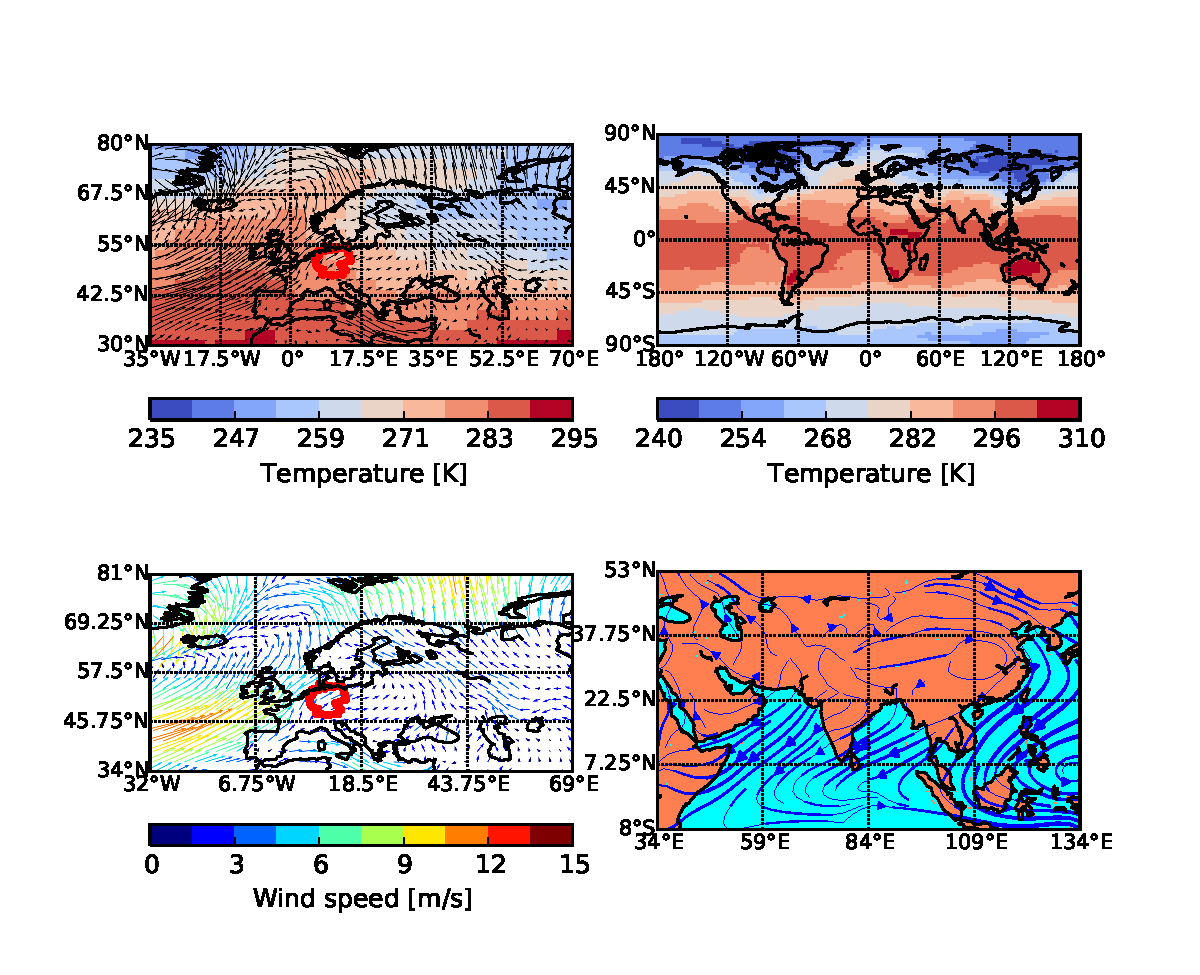
\includegraphics[width=0.9\textwidth]{figures/demo-plot-types.pdf}
	\caption{Demonstration of the different plot types with Pythons nc2map package}
	\label{fig:demo}
\end{figure}
This chapter is an introduction to the \gls{nc2map} Python module. The first section (\autoref{sec:modstruct}) deals with the general module structure, the second is a quick start showing how you can create your own maps (\autoref{sec:basic_init}) and the third is a more detailed description of the possibilities (\autoref{sec:init}).

Please also find demo scripts in the \lstinline|demo| directory of your \gls{nc2map} source files.

\section{A note about the module structure} \label{sec:modstruct}
As comparable with \lstinline|matplotlib|s axes (subplot) - figure structure, \gls{nc2map} consists of a basic class responsible for the plot (subclasses of \gls{MapBase}) and a coordinating class: \gls{MapsManager}. Each \gls{MapBase} instance thereby controls exactly one axes. A \gls{MapsManager} instance on the other hand controls multiple \gls{MapBase} instances. 

The most important \gls{MapsManager} subclass is the \gls{Maps} class which is not only designed to control many \gls{MapBase} instances but also colorbars, evaluations, output and updates to make everything interactive. Hence, the thing you probably will deal most with are instances of the \gls{Maps} class.

Furthermore, you will probably not deal with the \gls{MapBase} class, but rather with its subclasses. Those are \gls{FieldPlot}, to plot a two dimensional scalar field (e.g. temperature, see the upper row in figure \ref{fig:demo}) and \gls{WindPlot}, to visualize flows (e.g. wind or ocean currents, see the lower row in figure \ref{fig:demo}).

\section{Quick start} \label{sec:basic_init}
The simplest way how to plot open a NetCDF file and visualize it is with the \gls{Maps} class. If \lstinline|ncfile| is the variable containing the path to your NetCDF file, you can visualize the variables with
\begin{lstlisting}[label={lst:basic_init}, caption={Basic initialization of a \gls*{Maps} instance}]
	import nc2map
	ncfile = 'my-own-netcdf-file.nc'
	mymaps = nc2map.Maps(ncfile)     # initialize Maps instance
	mymaps.show()                    # show all figures
\end{lstlisting}
Or select specific variables via their name in the NetCDF file, e.g.
\begin{lstlisting}
	mymaps = nc2map.Maps(ncfile, vlst=['t2m', 'u'])
\end{lstlisting}
To visualize wind vectors, you can use the \lstinline|u| and \lstinline|v| keywords, e.g.
\begin{lstlisting}
	mymaps = nc2map.Maps(ncfile, u='u', v='v')
\end{lstlisting}
or if want to visualize only vector data without an underlying scalar field (e.g. temperature), you can do this by
\begin{lstlisting}
	mymaps = nc2map.Maps(ncfile, u='u', v='v', windonly=True)
\end{lstlisting}
You can then use the \gls{Maps.update} method to update the plot via formatoptions (see next \autoref{ch:fmt}). For example we can update the title of all plots via
\begin{lstlisting}
	mymaps.update(title='My test title of variable %(var)s.')
\end{lstlisting}
Here \lstinline|%(var)s| is replaced by the name of the specific variable that is shown in each plot, as it is used in the NetCDF file (actually you can use any meta data from the variables in the NetCDF file, see \autoref{sec:labels}). You can also update only specific \gls{MapBase} instances by using any of the meta attributes (e.g. \gls{time}, or \gls{level}, or \gls{var}) or directly via the instance specific attribute \gls{name}.

Hence let's say we only want to update the temperature (stored in variable \lstinline|t2m|) and zonal wind (stored in variable \lstinline|u|). Then we can update these \gls{MapBase} instances via
\begin{lstlisting}
	mymaps.update(title='My test title of variable %(var)s.', 
	              vlst=['t2m', 'u'])
\end{lstlisting}
For a detailed usage of the \gls{Maps.update} method please refer to the python built-in \lstinline|help| function.

Another possibility (see also next \autoref{sec:init}) would be to include the \glspl{fmt} directly in the initialization by the use of the \glssymbol{fmt} keyword via a dictionary
\begin{lstlisting}
	import nc2map
	ncfile = 'my-own-netcdf-file.nc'
	fmt = {'title': 'My test title of variable %(var)s.'}
	mymaps = nc2map.Maps(ncfile, fmt=fmt)  # initialize Maps instance
	mymaps.show()                 	       # show all figures
\end{lstlisting}
There are some demo scripts in the demo directory of your nc2map distribution which may show you some possible applications.

\section{Initializing a \texttt{nc2map.Maps} instance} \label{sec:init}
\subsection{How to specify the NetCDF files} \label{sec:init_nc}
\gls{nc2map} is primarily designed to plot NetCDF files, however it might be extended in the future (e.g. for GeoTiff files). You can simply pass in one single NetCDF file, use wildcards (e.g. $^*$ or ?) or a list of NetCDF files.
\begin{description}
	\item[One single file:] Simply use the file name, e.g. 
		\begin{lstlisting}
			mymaps = nc2map.Maps('my-netcdf-file.nc')|
		\end{lstlisting}
	\item[Using wild cards:] Same as with a single file name, e.g. 
		\begin{lstlisting}
			mymaps = nc2map.Maps('my-*-file.nc')
		\end{lstlisting}
	\item[Using multiple files:] Simply use a list of file names, e.g. 
	\begin{lstlisting}
		mymaps = nc2map.Maps(['my-netcdf-file1.nc', 'my-netcdf-file2.nc'])
	\end{lstlisting}
\end{description}
By default, \glssymbol{Maps} uses the \lstinline|netCDF4.Dataset| to visualize a single NetCDF file and the \lstinline|netCDF4.MFDataset| to visualize multiple NetCDF files. You can set manually which of the above classes is used via the \lstinline|mode| key word (\glslink{NCReader}{\lstinline|mode='NCReader'|} of \glslink{MFNCReader}{\lstinline|mode='MFNCReader|}) in the initialization of a \gls{Maps} instance. \\
Furthermore, instead of passing in the NetCDF file (or a list of NetCDF files), you can initialize the \gls{Maps} instance via setting the \lstinline|ncfile| equal to a dictionary, e.g.
\begin{lstlisting}
	mymaps = nc2map.Maps({'filename': 'my-netcdf-file.nc', 'mode': 'a'})
\end{lstlisting}
to open the NetCDF file in an editor mode. The key-value pairs of the dictionary are then assumed to represent the keyword arguments used for the initialization of the \glssymbol{ArrayReader} instance. \\
Finally you can also set the \lstinline|ncfile| keyword with an already existing \gls{reader} instance.


\subsection{Specifying what to plot via \glspl*{dimsidentifier}} \label{sec:init_dims}
The \gls{Maps} class takes a bunch of possible keywords for the initialization (see \lstinline|help(nc2map.Maps.__init__)| method for details). We already saw in listing \ref{lst:basic_init}, how to generally visualize a NetCDF file. However those commands would show all variables at the first time step, level, etc., which is maybe not desired. Therefore we can use the dimensions in the NetCDF file to be more specific. Which dimensions there are, depends on your specific NetCDF file. During the initialization of a \gls{Maps} instance, you can set any dimension you want, e.g.
\begin{lstlisting}
	# variables 't2m' and 'u' at the 2nd time step for 1st and 2nd level
	mymaps = nc2map.Maps(ncfile, vlst=['t2m', 'u'], time=1, level=[0, 1])
\end{lstlisting}
This will open 4 maps in total and assign automatically generated names \lstinline|mapo0, mapo1, mapo2| and \lstinline|mapo3| to the generated \gls{MapBase} instances. Note that for any dimension you specify in this way that is iterable\footnote{iterables in python are everything that does not raise an Error when using the built-in \lstinline|iter| function. The most prominent example are \lstinline|list|s (e.g. \lstinline|[1, 2, 3]|, or \lstinline|range(5)| or \lstinline|xrange(5)|).}, one \gls{MapBase} instance is created. Hence,
\begin{lstlisting}
	mymaps = nc2map.Maps(ncfile, vlst=['t2m', 'u'], time=range(5), level=[0, 1])
\end{lstlisting}
would create 20 maps in total (not recommended because far too much!).

Therefore, you can be more specific, by using the \glspl{name} keyword in the initialization of the \gls{Maps} instance and a dictionary. This might look like
\begin{lstlisting}
	names = {'mymap1': {'time': 1},
	         'mymap2': {'time': 1, 'level': 1}}
    mymaps = nc2map.Maps(ncfile, names=names)
\end{lstlisting}
and opens exactly two maps, one with \gls{time}\lstinline|=1| and \gls{level}\lstinline|=0| and one with \gls{time}\lstinline|=1| and \gls{level}\lstinline|=1|. This may also be useful if your variables in the NetCDF file have different dimensions.

If you do not use the \glspl{name} keyword as a dictionary but instead give another iterable (or a string with \lstinline|'{0}'| in it, e.g. \lstinline|mymodel{0}|), those will be used as names for the \gls{MapBase} instances, where the \lstinline|'{0}'| will be replaced by a counter. However, maybe it is not so useful to define your own names, but rather to give some meta attributes directly to the \gls{MapBase} via the \lstinline|meta| key. As an example
\begin{lstlisting}[label={lst:own_meta}, caption={Assigning your own meta informations}]
	mymaps = nc2map.Maps(ncfile, meta={'model': 'my first model'})
	mymaps.addmap(ncfile, meta={'model': 'my second model'})
\end{lstlisting}
will allow you to later address the \gls{MapBase} instances you want via the \lstinline|model| key, e.g.
\begin{lstlisting}
	model_maps1 = mymaps.get_maps(model='my first model')
	model_maps2 = mymaps.get_maps(model='my second model')
\end{lstlisting}
Instead of setting \lstinline|time| to 1, you can also use the time information in the NetCDF file (see \autoref{sec:time})

Those dimensions can also be changed via the \lstinline|Maps.update| method. For example
\begin{lstlisting}
	mymaps.update(fmt={'time': 1}, time=0)
\end{lstlisting}
will update all maps that currently show the first time step to the second. For time however, you can also use the \gls{Maps.nextt} and \gls{Maps.prevt} methods.

The function that is used in the initialization to add new maps to the \gls{Maps} instance, is the \gls{MapsManager.addmap} method. Hence, to add another map to the \gls{Maps} instance, you can simply use
\begin{lstlisting}
    mymaps.addmap(ncfile, ...)
\end{lstlisting}
Furthermore there is the possibility to make one dimensional line plots with data from the NetCDF file. The syntax is somewhat similar, e.g.:
\begin{lstlisting}
	mymaps = nc2map.Maps(ncfile, vlst=['t2m', 'u'], level=[0, 1], lat=0, lon=0, linesonly=True)
\end{lstlisting}
will draw lines over all time steps in the NetCDF file into one subplot for the first and second level. The corresponding method that is used is the \gls{MapsManager.addline} method.

\subsection{Specifying how to plot via \gls*{fmt} keywords}
There exist over 60 formatoptions, that can be used to exactly control the appearance of your plot. Each formatoption can be set with one single keyword (see next \autoref{ch:fmt}).

As stated already in \autoref{sec:basic_init}, you can give \glspl{fmt} directly to the initialization of the \gls{Maps} instance without using the \gls{Maps.update} method. These can be done via simply setting up a dictionary with \gls{fmt} keywords like
\begin{lstlisting}
	fmt = {'title': 'my test title',
	       'cmap': 'RdBu'}
\end{lstlisting}
However this would set the title for all variables, all time steps and all levels, in other words for all \gls{MapBase} instances that are controlled by the \gls{Maps} instance. But sometimes we do not want the same formatoptions for each \gls{MapBase} instance. For example we maybe want a colormap going from red to blue for precipitation (e.g. \lstinline|pyplots| \lstinline|'RdBu_r'| colormap) and a colormap going from blue to red for temperature (e.g. \lstinline|pyplots| \lstinline|'RdBu_r'| colormap). Therefore we can set up the \glspl{fmt} dictionary more specifically. In our case for example let's assume that precipitation is stored in the variable \lstinline|precip| and temperature in the variable \lstinline|t2m|. Our \gls{fmt} dictionary for the initialization will then be
\begin{lstlisting}
	fmt = {'title': ' %(long_name)s',
	       't2m': {'cmap': 'RdBu_r'},
	       'precip': {'cmap': 'RdBu'}
	      }
\end{lstlisting}
i.e. we used the variable identifier as a key in the \glssymbol{fmt} dictionary whose value is another \glssymbol{fmt} dictionary. Please note that the \lstinline|'title'| \gls{fmt} is set outside of the variable specific dictionaries which means that this is used as a default value for all \gls{MapBase} instances in the \gls{Maps} instance. However, since we refer here to the \lstinline|long_name| attribute inside the NetCDF file, the titles will not be the same. Hence setting up the above dictionary like
\begin{lstlisting}
	fmt = {'title': 'my test title',
	       't2m': {'cmap': 'RdBu_r',
	               'title': 'Another title'},
	       'precip': {'cmap': 'RdBu'}
	      }
\end{lstlisting}
would result in a title being \enquote{Another title} for all \lstinline|t2m| \gls{MapBase} instances and \enquote{my test title} for all the others (e.g. \lstinline|precip|).

This syntax does not only work for variables but also slightly modified for \glspl{time}, \glspl{level} and \glspl{name}. The \gls{time} step furthermore has to come with a leading \lstinline|t| followed by the time step as string, whereas the \gls{level} has to come with a leading \lstinline|l| followed by the vertical step as string. Hence
\begin{lstlisting}
	fmt = {'t0': {'title': 'This applies only for the 0-th time step'}}
\end{lstlisting}
will only modify the titles of \gls{MapBase} instances with \gls{time}\lstinline| == 0| and
\begin{lstlisting}
	fmt = {'l0': {'title': 'This applies only for the 0-th level'}}
\end{lstlisting}
will only modify the titles of \gls{MapBase} instances with \gls{level}\lstinline| == 0|.
Finally 
\begin{lstlisting}
	fmt = {'mapo0': {'title': 'This applies only for the 0-th level'}}
\end{lstlisting}
will only modify the title of the \gls{MapBase} instance with the name \lstinline|mapo0|.

Furthermore the dictionaries can be nested, where the order of hierarchy is 
\begin{equation*}
\text{\gls{name}} \succ \text{\gls{var}} \succ \text{\gls{time}} \succ \text{\gls{level}}. 
\end{equation*}
As an example look into listing \ref{lst:nested_fmt}.
\begin{lstlisting}[label={lst:nested_fmt}, caption={Example of how to define a nested formatoptions dictionary.},float,floatplacement=H]
	default_title = 'Default title'
	mapo0_title = 'Title used for mapo0'
	t2m_title = 'Default title for t2m variable'
	t2m_t2_title = 'Title for third time step of t2m variable'
	t1_title = 'Default title for second time step'

	fmt = {'title': default_title,
	       'mapo0': {'title': mapo0_title},
	       't2m': {'title': t2m_title,
	               't2': {'title': t2m_t2_title}},
	       't1': {'title': t1_title}
	       }
\end{lstlisting}
Here we set the title for the \gls{MapBase} instance with \gls{name} \lstinline|== mapo0| to \lstinline|mapo0_title|, the title for all \gls{MapBase} instances with \gls{time} \lstinline|== 1| and \gls{var} \lstinline|!= 't2m'| to \lstinline|t1_title|, the title for all time step and levels with \gls{var} \lstinline|== 't2m'| and \gls{time} \lstinline|!= 2| to \lstinline|t2m_title| and finally for \gls{var} \lstinline|== 't2m'| and \gls{time} \lstinline|== 2| to \lstinline|t2m_t2_title|.


\section{Output methods} \label{sec:output}
There are several methods of the \gls{Maps} class to save what you created:
\begin{description}
	\item[\glslink{Maps.output}{\texttt{output}}:] Save all (or some) figures into one (or more) \lstinline|pdf| files, \lstinline|png|s, \lstinline|jpg|s, etc.
	\item[\glslink{Maps.make_movie}{\texttt{make\_movie}}:] Make a movie (e.g. \lstinline|.gif| or \lstinline|.mp4|) of your \gls{MapBase} instances.
	\item[\glslink{Maps.save}{\texttt{save}}:] Creates a python script that initializes the \gls{Maps} instance in its current state (including all\gls{MapBase} and \gls{LinePlot} instances and their \glspl{fmt}.) This file can then be loaded by the \gls{nc2map.load} function to restore the \gls{Maps} instance.
\end{description}


\section{Helper functions accessing the documentation} \label{sec:helper}
There are several helper functions to cope with the visualization of your data:
\begin{description}
	\item[\glslink{show_colormaps}{\texttt{show\_colormaps}}:] This function can be used to show all the colormaps that are predefined by the \gls{nc2map} module and \lstinline|pyplot|. You can also use it to visualize your own created colormap to see, how it will finally look like.
	\item[\glslink{show_fmtkeys}{\texttt{show\_fmtkeys}:}] This function shows the possible \gls{fmt} keywords or checks whether the the keywords specified by the user are possible.
	\item[\glslink{show_fmtdocs}{\texttt{show\_fmtdocs}:}] This function shows the possible \gls{fmt} keywords or checks whether the the keywords specified by the user are possible, plus their documentation.
	\item[\glslink{get_fmtkeys}{\texttt{get\_fmtkeys}:}] This function returns a list of possible \gls{fmt} keywords as strings, or checks whether the the keywords specified by the user are possible.
	\item[\glslink{get_fmtdocs}{\texttt{get\_fmtdocs}:}] This function returns a dictionary with the possible \gls{fmt} keywords as keys and their documentation as value.
	\item[\glslink{nc2map.get_fnames}{\texttt{get\_fnames}}:] Shows the possible field names in the default shape file for the \hyperref[item:lineshapes]{\lstinline|lineshapes|} keyword (you can also use other shape files, see the corresponding function in the \gls{shp_utils} function).
	\item[\glslink{nc2map.get_unique_vals}{\texttt{get\_unique\_vals}}:] Shows the values in the default shape file for the \hyperref[item:lineshapes]{\lstinline|lineshapes|} keyword (you can also use other shape files, see the corresponding function in the \gls{shp_utils} function).
\end{description}

\section{Automatical labelling} \label{sec:labels}
One very useful feature of the \gls{nc2map} module is that you can very easily implement the meta data information of the NetCDF file in your plot. There are some labels (e.g. \hyperref[item:clabel]{clabel}, \hyperref[item:title]{title}, \hyperref[item:text]{text}, etc., see table \ref{tab:fmt_keys}) which you can set with strings that are then displayed on the plot. The following subsections describe how to use the text-like meta information of the NetCDF file in your labels (\autoref{sec:labels_text}) and how to display the time information (\autoref{sec:labels_time}).

\subsection{Using text meta data} \label{sec:labels_text}
For example let's take the variable \lstinline|t2m|. Of course you could simply set \hyperref[item:title]{\lstinline|title|}\lstinline|='Plot of t2m'| but why should you double your work if that variable is stored in the NetCDF file anyway? Therefore a much easier solution is setting \hyperref[item:title]{\lstinline|title|}\lstinline|='Plot of %(var)s'|. In fact in all labels you can replace any meta information stored (e.g. \lstinline|long_name|) by \lstinline| %(long_name)s|.

Common meta data keys are:
\begin{description}
	\item[\glslink{var}{\texttt{var}}:] Name of the variable as stored in the NetCDF file (e.g. \lstinline|t2m|)\footnote{\label{foot:MapBasedims}This information is always stored in the \gls{MapBase} instance, it is not a meta data information in the NetCDF file}
	\item[\texttt{standard\_name}:] Standard name of the variable (e.g. \lstinline|evapotranspiration| for variable \lstinline|evspsbl|)
	\item[\texttt{long\_name}:] Long name of the variable (e.g. \lstinline|Temperature|)
	\item[\texttt{units}:] Unit of the variable (e.g. \lstinline|deg C|)
	\item[\glslink{time}{\texttt{time}}:] Time step
	\item[\glslink{level}{\texttt{level}}:] Number of the vertical level
	\item[\glslink{name}{\texttt{name}}:] Name of the \gls{MapBase} instance$^\text{\ref{foot:MapBasedims}}$
\end{description}
Anyway, which meta data key is stored in a NetCDF file is determined by the NetCDF file (i.e. by the conscientiousness of the creator of the file). You can access the meta data keys via the \gls{MapBase.meta} property of the specific \gls{MapBase} instance. E.g. if you want to see the meta information of the variable \lstinline|t2m|, simply use
\begin{lstlisting}
	mymaps = nc2map.Maps('my-own-netcdf-file.nc', vlst='t2m')
	print mymaps.get_maps(vlst='t2m')[0].meta
\end{lstlisting}
Another possibility is to use the \gls{MapsManager.get_label_dict} method of the \gls{Maps} instance via
\begin{lstlisting}
	mymaps = nc2map.Maps('my-own-netcdf-file.nc', vlst='t2m')
	print mymaps.get_label_dict(*mymaps.get_maps(vlst='t2m'))
\end{lstlisting}
or the \gls{MapsManager.meta} property.

\subsection{Displaying the time} \label{sec:labels_time}
As we saw in the previous \autoref{sec:labels_text}, one possibilty to display the time step is via \lstinline| %(|\gls{time}\lstinline|)s| in our labels. However, one of the great advantages of NetCDF files is that they (almost always) follow the CF-conventions\footnote{\url{http://cfconventions.org/}} and store the time data in relative time units (e.g. \lstinline|days since 1992-10-8 15:15:42.5 -6:00|) or at least in absolute time units (\lstinline|day as %Y%m%d.%f|). \gls{nc2map} interpretes those two units and uses the python \lstinline|datetime| module to display the information in the labels. Hence to display the time of your \gls{MapBase} instance, you can use all format strings suitable with the \lstinline|strftime| function of the \lstinline|datetime.datetime| module\footnote{For a list of format strings see \href{https://docs.python.org/2/library/datetime.html\#strftime-and-strptime-behavior}{\nolinkurl{https://docs.python.org/2/library/datetime.html}}}. For example lets assume that my \gls{MapBase} instance shows the variable \lstinline|t2m| on the 2$^\text{nd}$ of March, 2015. Then setting my title as \hyperref[item:title]{\lstinline|title|}\lstinline|=' %(var)s in %B, %Y'| would result in the title \lstinline|'t2m in March, 2015'| (or {\footnotesize \texttt{'t2m in M\"arz, 2015'}} if you are in Germany).

	% !TeX root = ../user_manual.tex
\chapter{NetCDF restrictions and dimension handling}
The \gls{nc2map} module is designed to very flexible. Therefore in principle every NetCDF file can be read. You can have as many dimensions in your NetCDF file as you want and you can name them as you want. However, only one can always be regarded as one of the special dimensions latitude, longitude, time and level. In detail:
\begin{enumerate}
	\item Your NetCDF file should only have one longitude variable and one latitude variable and the data of this dimensions have to be stored in two different variables
	\item Only one variable can be considered as the variable for the time dimension
	\item Only one variable can be considered as the variable for the level dimension
\end{enumerate}
You can tell the \gls{reader} at the initalization, what the \lstinline|levelnames| are it shall look for, the \lstinline|timenames|, the \lstinline|lonnames| and the \lstinline|latnames|. Those keywords can also be set at the initialization of a \gls{Maps} instance. (see \lstinline|help(nc2map.Maps)| and \lstinline|help(nc2map.readers.ReaderBase)|).

\section{Using the time information in the NetCDF file} \label{sec:time}
Concerning the time dimension, it is recommended to use relative or absolute time units. If the time information in the \gls{reader} (i.e. NetCDF file) is stored in relative (e.g. hours since ...) or absolute (day as \%Y\%m\%d.f) units, strings like \lstinline|%Y| for year or \lstinline|%m| for the month as given by the python datetime package in labels like \hyperref[item:title]{title}, \hyperref[item:text]{text}, etc., are also replaced by the specific time information. Furthermore you can then select the time step not only via the time step explicitly (i.e. the integer), but by the time information. You can then either use a string in isoformat, e.g. \lstinline|'1979-02'| for February 1979 or \lstinline|'1979-02-01T18:45'| for February 1st, 1979 at 18:45 in the evening, a \lstinline|numpy.datetime64| instance or a \lstinline|datetime.datetime| instance.
	% !TeX root = ../user_manual.tex
\chapter{Interactive usage} \label{ch:interactive}
One, or maybe the most important feature of the \gls{nc2map} module is it's capability for an interactive usage. You do not have to run the same script again and again but can use \lstinline|python| or \lstinline|ipython| (or any other python shell) to modify your plots at run time. I recommend to use the interactive python shell \lstinline|ipython|, because it also has the \lstinline| %save| magic to save your commands as a script.

However, the updating process is rather simple via the \glssymbol{Maps.update} method. You can also find a demo script in the \lstinline|nc2map/demo| directory, but you learn it the best, if you simply try it by yourself. The \gls{Maps.update} method takes every
formatoption keyword (see next \autoref{ch:fmt}) as keyword and any meta attribute in your \gls{MapBase} instance as a selector.
For example
\begin{lstlisting}[label={lst:update_var}, caption={Update formatoptions variable specific}]
	mymaps.update(var='t2m', cmap='RdBu_r')
\end{lstlisting}
will update the colormap of all \gls{MapBase} instances showing the NetCDF variable \lstinline|t2m|. The same works for own created meta data, e.g. coming back to listing \ref{lst:own_meta},
\begin{lstlisting}
	mymaps.update(model='my first model', lonlatbox='Europe')
\end{lstlisting}
will update the plot of all \gls{MapBase} instances that were created with the \lstinline|'my first model'| flag to focus on Europe, whereas all the others keep untouched. The same works for meta informations stored in the variable of the NetCDF file, e.g.
\begin{lstlisting}
	mymaps.update(long_name='Temperature', cmap='RdBu_r')
\end{lstlisting}
will have the same effect as listing \ref{lst:update_var}. You can also pass in a list of meta attributes instead of strings, e.g
\begin{lstlisting}
	mymaps.update(model=['my first model', 'my second model'], cmap='RdBu')
\end{lstlisting}

	% !TeX root = ../user_manual.tex
\chapter{\Glspl*{fmt}} \label{ch:fmt}
The basic control feature for the appearance of the plot are the \gls{fmt} keywords, usually identified by the \glssymbol{fmt} key, for example in the initialization of a \gls{Maps} instance or in the \glssymbol{Maps.update} method\footnote{However, you can either give the formatoptions directly as keyword argument to the \gls{Maps.update} method or as dictionary via the \glssymbol{fmt} key.}. The possible formatoptions depend on what you are plotting. A \gls{FieldPlot} (upper row in figure \ref{fig:demo}) for example has the possible formatoptions shown in table \ref{tab:fmt_keys}. A \gls{WindPlot} (lower row in figure \ref{fig:demo}) additionally has the keywords shown in table \ref{tab:windfmt_keys} and simple plots (\gls{LinePlot} instances) have the formatoptions shown in table \ref{tab:simplefmt_keys}. 

The following sections are automatically generated from the \gls{nc2map} module. They show the documentation of the \gls{fmt} keys, however there are some helper functions to display possible keys and their usage inside python: \glssymbol{show_fmtkeys} and \glssymbol{show_fmtdocs} (see \autoref{sec:helper}).\footnote{Hint: \gls{show_fmtkeys} can also be used to look how to exactly spell the formatoption keyword you want to use.}

\begin{table}
    \centering
    \captionabove{List of formatoption keywords}
    \label{tab:fmt_keys}
    \begin{tabular}{|p{0.18\textwidth}|p{0.18\textwidth}|p{0.18\textwidth}|p{0.18\textwidth}|p{0.18\textwidth}|}
        \hline
        \hyperref[item:axiscolor]{axiscolor}           & \hyperref[item:bounds]{bounds}                 & \hyperref[item:clabel]{clabel}                 & \hyperref[item:cmap]{cmap}                     & \hyperref[item:countries]{countries}           \\
        \hline
        \hyperref[item:cticksize]{cticksize}           & \hyperref[item:ctickweight]{ctickweight}       & \hyperref[item:enable]{enable}                 & \hyperref[item:extend]{extend}                 & \hyperref[item:figtitle]{figtitle}             \\
        \hline
        \hyperref[item:figtitlesize]{figtitlesize}     & \hyperref[item:figtitleweight]{figtitleweight} & \hyperref[item:fontsize]{fontsize}             & \hyperref[item:fontweight]{fontweight}         & \hyperref[item:grid]{grid}                     \\
        \hline
        \hyperref[item:labelsize]{labelsize}           & \hyperref[item:labelweight]{labelweight}       & \hyperref[item:land_color]{land\_color}        & \hyperref[item:latlon]{latlon}                 & \hyperref[item:lineshapes]{lineshapes}         \\
        \hline
        \hyperref[item:lonlatbox]{lonlatbox}           & \hyperref[item:lsm]{lsm}                       & \hyperref[item:mask]{mask}                     & \hyperref[item:maskbetween]{maskbetween}       & \hyperref[item:maskgeq]{maskgeq}               \\
        \hline
        \hyperref[item:maskgreater]{maskgreater}       & \hyperref[item:maskleq]{maskleq}               & \hyperref[item:maskless]{maskless}             & \hyperref[item:meridionals]{meridionals}       & \hyperref[item:merilabelpos]{merilabelpos}     \\
        \hline
        \hyperref[item:ocean_color]{ocean\_color}      & \hyperref[item:paralabelpos]{paralabelpos}     & \hyperref[item:parallels]{parallels}           & \hyperref[item:plotcbar]{plotcbar}             & \hyperref[item:proj]{proj}                     \\
        \hline
        \hyperref[item:rasterized]{rasterized}         & \hyperref[item:text]{text}                     & \hyperref[item:ticklabels]{ticklabels}         & \hyperref[item:ticks]{ticks}                   & \hyperref[item:ticksize]{ticksize}             \\
        \hline
        \hyperref[item:tickweight]{tickweight}         & \hyperref[item:tight]{tight}                   & \hyperref[item:title]{title}                   & \hyperref[item:titlesize]{titlesize}           & \hyperref[item:titleweight]{titleweight}       \\
        \hline
        \hyperref[item:windplot]{windplot}             &  &  &  &  \\
        \hline
    \end{tabular}
\end{table}
\begin{table}
    \centering
    \captionabove{List of wind specific formatoption keywords}
    \label{tab:windfmt_keys}
    \begin{tabular}{|p{0.18\textwidth}|p{0.18\textwidth}|p{0.18\textwidth}|p{0.18\textwidth}|p{0.18\textwidth}|}
        \hline
        \hyperref[item:scale]{scale}             & \hyperref[item:arrowstyle]{arrowstyle}   & \hyperref[item:density]{density}         & \hyperref[item:color]{color}             & \hyperref[item:lengthscale]{lengthscale} \\
        \hline
        \hyperref[item:reduceabove]{reduceabove} & \hyperref[item:streamplot]{streamplot}   & \hyperref[item:arrowsize]{arrowsize}     & \hyperref[item:enable]{enable}           & \hyperref[item:linewidth]{linewidth}     \\
        \hline
        \hyperref[item:clabel]{clabel}           &  &  &  &  \\
        \hline
    \end{tabular}
\end{table}
\begin{table}
    \centering
    \captionabove{List of LinePlot specific formatoption keywords}
    \label{tab:simplefmt_keys}
    \begin{tabular}{|p{0.18\textwidth}|p{0.18\textwidth}|p{0.18\textwidth}|p{0.18\textwidth}|p{0.18\textwidth}|}
        \hline
        \hyperref[item:axiscolor]{axiscolor}           & \hyperref[item:enable]{enable}                 & \hyperref[item:figtitle]{figtitle}             & \hyperref[item:figtitlesize]{figtitlesize}     & \hyperref[item:figtitleweight]{figtitleweight} \\
        \hline
        \hyperref[item:fontsize]{fontsize}             & \hyperref[item:fontweight]{fontweight}         & \hyperref[item:grid]{grid}                     & \hyperref[item:labelsize]{labelsize}           & \hyperref[item:labelweight]{labelweight}       \\
        \hline
        \hyperref[item:legend]{legend}                 & \hyperref[item:scale]{scale}                   & \hyperref[item:text]{text}                     & \hyperref[item:ticksize]{ticksize}             & \hyperref[item:tickweight]{tickweight}         \\
        \hline
        \hyperref[item:tight]{tight}                   & \hyperref[item:title]{title}                   & \hyperref[item:titlesize]{titlesize}           & \hyperref[item:titleweight]{titleweight}       & \hyperref[item:xlabel]{xlabel}                 \\
        \hline
        \hyperref[item:xlim]{xlim}                     & \hyperref[item:xrotation]{xrotation}           & \hyperref[item:xticklabels]{xticklabels}       & \hyperref[item:xticks]{xticks}                 & \hyperref[item:ylabel]{ylabel}                 \\
        \hline
        \hyperref[item:ylim]{ylim}                     & \hyperref[item:yrotation]{yrotation}           & \hyperref[item:yticklabels]{yticklabels}       & \hyperref[item:yticks]{yticks}                 &  \\
        \hline
    \end{tabular}
\end{table}


\section{Basemap and axes formatoptions}
\begin{description}
    \item[\gls*{figtitlesize}:] \label{item:figtitlesize}  string or float (Default: 12). Defines the size of the subtitle of the figure (see fontsize for possible values). This is the title of this specific axes! For the title of the figure see figtitlesize
    \item[\gls*{text}:] \label{item:text}  String, tuple or list of tuples (x,y,s[,coord.-system][,options]]) (Default: []).
\begin{itemize}
    \item If string s: this will be used as (1., 1., s, {\enquote{ha}: \enquote{right}}) (i.e. a string in the upper right corner of the axes).
    \item If tuple or list of tuples, each tuple defines a text instance on the plot. 0$\leq$x, y$\leq$1 are the coordinates. The coord.-system can be either the data coordinates (default, \enquote{data}) or the axes coordinates (\enquote{axes}) or the figure coordinates (\enquote{fig}). The string s finally is the text. options may be a dictionary to specify format the appearence (e.g. \enquote{color}, \enquote{fontweight}, \enquote{fontsize}, etc., see matplotlib.text.Text for possible keys). To remove one single text from the plot, set (x,y,'') for the text at position (x,y); to remove all set text=[]. Metadata keys (var, time, level, or netCDF attributes like long\_name, units, ...) maybe replaced via \%(key)s. If the time information in the reader (i.e. NetCDF file) is stored in relative (e.g. hours since ...) or absolute (day as \%Y\%m\%d.f) units, directives like \%Y for year or \%m for the month as given by the python datetime package, are also replaced by the specific time information. There are furthermore some special keys which are replaced when you insert '{key}' in your text (e.g. {tinfo}). Those are tinfo: \%B \%d, \%Y. \%H:\%M dinfo: \%B \%d, \%Y Those special keys are defined in the nc2map.defaults.texts[\enquote{labels}] dictionary.
\end{itemize}

    \item[\gls*{lsm}:] \label{item:lsm}  Boolean (Default: True). If True, the continents will be plottet.
    \item[\gls*{merilabelpos}:] \label{item:merilabelpos}  List of 4 values (Default: None) that control whether meridians are labelled where they intersect the left, right, top or bottom of the plot. For example labels=[1, 0, 0, 1] will cause meridians to be labelled where they intersect the left and bottom of the plot, but not the right and top.
    \item[\gls*{ticksize}:] \label{item:ticksize}  string or float (Default: small). Defines the size of the ticks (see fontsize for possible values)
    \item[\gls*{labelsize}:] \label{item:labelsize}  string or float (Default: medium). Defines the size of x- and y-axis labels (see fontsize for possible values)
    \item[\gls*{latlon}:] \label{item:latlon}  True/False (Default: True). Sets latlon keyword for basemap plot function (or not).
    \item[\gls*{figtitleweight}:] \label{item:figtitleweight}  Fontweight of the figure suptitle (Default: Defined by fontweight property). See fontweight above for possible values.
    \item[\gls*{titleweight}:] \label{item:titleweight}  Fontweight of the title (Default: Defined by fontweight property). See fontweight above for possible values. This is the title of this specific axes! For the title of the figure see figtitleweight
    \item[\gls*{lonlatbox}:] \label{item:lonlatbox}  1D-array [lon1,lon2,lat1,lat2], string (or pattern), or dictionary (Default: global, i.e. [-180.0, 180.0, -90.0, 90.0] for proj==\enquote{cyl} and Northern Hemisphere for \enquote{northpole} and Southern for \enquote{southpole}). Selects the region for the plot.
\begin{itemize}
    \item If string this will be compiled as a pattern to match any of the keys in nc2map.defaults.lonlatboxes (it contains longitude-latitude definitions for countries and continents). E.g. to focus on Germany, set lonlatbox=\enquote{Germany}. To focus on Africa, set lonlatbox=\enquote{Africa}. To focus on Germany, France and Italy, set lonlatbox='Germany|France|Italy'.
    \item If dictionary possible keys are
\begin{itemize}
        \item \enquote{ifile} to give an input shapefile (if not set, use the shapes from the default shape file located at /home/chilipp/Dokumente/myplots-scripts/nc2map/data/countries\_and\_continents\_vmap0 This Shapefile is based upon the bnd-political-boundary-a.shp shapes from the Vmap0 Dataset from GIS-Lab (http://gis-lab.info/qa/vmap0-eng.html), accessed May 2015.
        \item any field name in the input shape file (see nc2map.get\_fnames and nc2map.get\_unique\_vals function) to select specific shapes
\end{itemize}
\end{itemize}


    \item[\gls*{labelweight}:] \label{item:labelweight}  Fontweight of axis labels (Default: Defined by fontweight property). See fontweight above for possible values.
    \item[\gls*{mask}:] \label{item:mask}  array (x[, var][, num]) (Default: None). The first entry must be a string for a netCDF file or a nc2map.readers.ArrayReader instance, the second entry might be the name of the variable in the mask file to read in, the number at the end defines the values where to mask (if not given, mask everywhere where the mask is 0)
    \item[\gls*{tight}:] \label{item:tight} Boolean (Default: False). Make tight\_layout after plotting if True.
    \item[\gls*{proj}:] \label{item:proj}  string (\enquote{cyl}, \enquote{robin}, \enquote{northpole}, \enquote{southpole}) or dictionary (Default: cyl). Defines the options for the projection used for the plot. If string, Basemap is set up automatically with settings from lonlatbox, if dictionary, these are the keyword arguments passed to mpl\_toolkits.basemap.Basemap initialization.
    \item[\gls*{titlesize}:] \label{item:titlesize}  string or float (Default: large). Defines the size of the title (see fontsize for possible values)
    \item[\gls*{parallels}:] \label{item:parallels}  1D-array or integer (Default: 5). Defines the lines where to draw parallels. Possible types are
\begin{itemize}
    \item 1D-array: manually specify the location of the parallels
    \item integer: Gives the number of parallels between maximal and minimal lattitude (including max- and minimum line)
\end{itemize}

    \item[\gls*{fontweight}:] \label{item:fontweight}  A numeric value in the range 0-1000 or string (Default: None). Defines the fontweight of the ticks. Possible strings are one of \enquote{ultralight}, \enquote{light}, \enquote{normal}, \enquote{regular}, \enquote{book}, \enquote{medium}, \enquote{roman}, \enquote{semibold}, \enquote{demibold}, \enquote{demi}, \enquote{bold}, \enquote{heavy}, 'extra bold', \enquote{black}.
    \item[\gls*{paralabelpos}:] \label{item:paralabelpos}  List of 4 values (Default: None) that control whether parallels are labelled where they intersect the left, right, top or bottom of the plot. For example labels=[1, 0, 0, 1] will cause parallels to be labelled where they intersect the left and and bottom of the plot, but not the right and top.
    \item[\gls*{grid}:] \label{item:grid}  Enables the plotting of the grid on the axes if not None (Default: False).
    \item[\gls*{axiscolor}:] \label{item:axiscolor}  string or color for axis or dictionary (Default: {\enquote{top}: None, \enquote{right}: None, \enquote{bottom}: None, \enquote{left}: None}). If string or color this will set the default value for all axis. If dictionary, keys must be in [\enquote{right}, \enquote{left}, \enquote{top}, \enquote{bottom}] and the values must be a string or color to set the color for \enquote{right}, \enquote{left}, \enquote{top} or \enquote{bottom} specificly.
    \item[\gls*{ocean_color}:] \label{item:ocean_color}  color instance (Default: None). Specify the color of the ocean. Attention! Might reduce the performance a lot if multiple plots are opened! To not kill everything, use the MapBase.share.lsmask method of the specific MapBase instance.
    \item[\gls*{lineshapes}:] \label{item:lineshapes}  string, list of strings or dictionary. (Default: None). Draw polygons on the map from a shapefile.
\begin{itemize}
    \item If string or list of strings this will be seen as the values for the COUNTRY field in the default shapefile (see \enquote{ifile} below) and all matching polygons in this shape file will be merged.
    \item If dictionary possible keys are
\begin{itemize}
        \item \enquote{ifile} to give an input shapefile (if not set, use the shapes from the default shape file located at /home/chilipp/Dokumente/myplots-scripts/nc2map/data/countries\_and\_continents\_vmap0 This Shapefile is based upon the bnd-political-boundary-a.shp shapes from the Vmap0 Dataset from GIS-Lab (http://gis-lab.info/qa/vmap0-eng.html), accessed May 2015.
        \item \enquote{ofile} for the target shape file if specific shapes are selected or \enquote{dissolve} is set to False
        \item \enquote{dissolve}. True/False (Default: False). If True, all polygons will be merged into one single shape
        \item any field name in the input shape file (see nc2map.get\_fnames and nc2map.get\_unique\_vals function) to select specific shapes
        \item any other key (but the \enquote{name} key) which is finally passed to the readshapefile method (e.g. \enquote{color} or \enquote{linewidth})\\
 Each shape is uniquely defined through a key. If you use a dictionary d with the settings described above, you can set the key manually via {'my\_own\_key': d}. Otherwise a key like 'shape\%i' will automatically be assigned, where '\%i' depends on the number of already existing shapes.\\
 You can use these keys to remove a shape from the current plot by simply setting shapes='key\_to\_remove' (or whatever key you want to remove). Otherwise you can remove all drawn shapes with anything that evaluates to False (e.g. shapes=None). Please note that it might take a while to dissolve all polygons if \enquote{dissolve} is set to True and even to extract them if the shapefile is large. Therefore, if you use the shape on multiple plots, use the share.lineshapes method of the specific MapBase instance
\end{itemize}
\end{itemize}


    \item[\gls*{rasterized}:] \label{item:rasterized}  Boolean (Default: True). Rasterize the pcolormesh (i.e. the mapplot) or not.
    \item[\gls*{countries}:] \label{item:countries}  Boolean (Default: False). If True, draw country borders.
    \item[\gls*{title}:] \label{item:title}  string (Default: None). Defines the title of the plot. Metadata keys (var, time, level, or netCDF attributes like long\_name, units, ...) maybe replaced via \%(key)s. If the time information in the reader (i.e. NetCDF file) is stored in relative (e.g. hours since ...) or absolute (day as \%Y\%m\%d.f) units, directives like \%Y for year or \%m for the month as given by the python datetime package, are also replaced by the specific time information. There are furthermore some special keys which are replaced when you insert '{key}' in your text (e.g. {tinfo}). Those are tinfo: \%B \%d, \%Y. \%H:\%M dinfo: \%B \%d, \%Y Those special keys are defined in the nc2map.defaults.texts[\enquote{labels}] dictionary. This is the title of this specific axes! For the title of the figure see figtitle
    \item[\gls*{meridionals}:] \label{item:meridionals}  1D-array or integer (Default: 7). Defines the lines where to draw meridionals. Possible types are
\begin{itemize}
    \item 1D-array: manually specify the location of the meridionals
    \item integer: Gives the number of meridionals between maximal and minimal longitude (including max- and minimum line)
\end{itemize}

    \item[\gls*{land_color}:] \label{item:land_color}  color instance (Default: None). Specify the color of the land. 
    \item[\gls*{tickweight}:] \label{item:tickweight}  Fontweight of ticks (Default: Defined by fontweight property). See fontweight above for possible values.
    \item[\gls*{figtitle}:] \label{item:figtitle}  string (Default: None). Defines the figure suptitle of the plot.
    \item[\gls*{fontsize}:] \label{item:fontsize}  string or float (Default: None). Defines the default size of ticks, axis labels and title. Strings might be 'xx-small', 'x-small', \enquote{small}, \enquote{medium}, \enquote{large}, 'x-large', 'xx-large'. Floats define the absolute font size, e.g., 12
\end{description}

\section{Colorbar and colormap formatoptions}
\begin{description}
    \item[\gls*{plotcbar}:] \label{item:plotcbar}  String or list of possible strings (see below). Default: [\enquote{b}]. Determines where to plot the colorbar. Possibilities are \enquote{b} for at the bottom of the plot, \enquote{r} for at the right side of the plot, \enquote{sh} for a horizontal colorbar in a separate figure, \enquote{sv} for a vertical colorbar in a separate figure. For no colorbar use '', None, False, [], etc. A string may be a combination of multiple positions (e.g. \enquote{bsh} will draw a colorbar at the bottom of the plot and a separate horizontal one).
    \item[\gls*{extend}:] \label{item:extend}  string (\enquote{neither}, \enquote{both}, \enquote{min} or \enquote{max}) (Default: neither). If not \enquote{neither}, make pointed end(s) for out-of-range values. These are set for a given colormap using the colormap set\_under and set\_over methods.
    \item[\gls*{ctickweight}:] \label{item:ctickweight}  Fontweight of colorbar ticks (Default: Defined by fontweight property). See fontweight above for possible values.
    \item[\gls*{ticklabels}:] \label{item:ticklabels}  Array (Default: None). Defines the ticklabels of the colorbar
    \item[\gls*{bounds}:] \label{item:bounds}  1D-array, tuple or string (Default: (\enquote{rounded}, 11)). Defines the bounds used for the colormap. Possible types are
\begin{itemize}
    \item 1D-array: Defines the bounds directly by giving the values
    \item tuple (string, N): Compute the bounds automatically. N gives the number of increments whereas string can be one of the following strings
\begin{itemize}
        \item \enquote{rounded}: Rounds min and maxvalue of the data to the next 0.5-value with respect to its exponent with base 10 (i.e. 1.3e-4 will be rounded to 1.5e-4)
        \item \enquote{roundedsym}: Same as \enquote{rounded} but symmetric around zero using the maximum of the data maximum and (absolute value of) data minimum.
        \item \enquote{minmax}: Uses minimum and maximum of the data (without rounding)
        \item \enquote{sym}: Same as \enquote{minmax} but symmetric around 0 (see \enquote{rounded} and \enquote{roundedsym}).
\end{itemize}

    \item tuple (string, N, percentile): Same as (string, N) but uses the percentiles defined in the 1D-list percentile as maximum. percentile must have length 2 with [minperc, maxperc]
    \item string: same as tuple with N automatically set to 11.
\end{itemize}

    \item[\gls*{cticksize}:] \label{item:cticksize}  string or float (Default: medium). Defines the size of the colorbar ticks (see fontsize for possible values)
    \item[\gls*{cmap}:] \label{item:cmap}  string or colormap (e.g.matplotlib.colors.LinearSegmentedColormap) (Default: jet). Defines the used colormap. If cmap is a colormap, nothing will happen. Otherwise if cmap is a string, a colorbar will be chosen. Possible strings are
\begin{itemize}
    \item 'red\_white\_blue' (e.g. for symmetric precipitation colorbars)
    \item 'white\_red\_blue' (e.g. for asymmetric precipitation colorbars)
    \item 'blue\_white\_red' (e.g. for symmetric temperature colorbars)
    \item 'white\_blue\_red' (e.g. for asymmetric temperature colorbars)
    \item any other name of a standard colorbar as provided by pyplot (e.g. \enquote{jet},\enquote{Greens},\enquote{binary}, etc.). Use function nc2map.show\_colormaps to visualize them.
\end{itemize}

    \item[\gls*{ticks}:] \label{item:ticks}  1D-array or integer (Default: None). Define the ticks of the colorbar. In case of an integer i, every i-th value of the default ticks will be used.
\end{description}

\section{Masking properties}
\begin{description}
    \item[\gls*{maskgreater}:] \label{item:maskgreater}  Float (Default: None). All data greater than this value is masked (see also maskgeq)
    \item[\gls*{maskbetween}:] \label{item:maskbetween}  Tuple or list (Default: None). Pair (min, max) between which the data shall be masked
    \item[\gls*{maskless}:] \label{item:maskless}  Float (Default: None). All data less than this value is masked (see also maskleq)
    \item[\gls*{maskleq}:] \label{item:maskleq}  Float (Default: None). All data less or equal than this value is masked (see also maskless)
    \item[\gls*{maskgeq}:] \label{item:maskgeq}  Float (Default: None). All data greater or equal than this value is masked (see also maskgreater)
\end{description}

\section{Windplot specific formatoptions}
\begin{description}
    \item[\gls*{arrowsize}:] \label{item:arrowsize}  float (Default: 1.0). Defines the size of the arrows
    \item[\gls*{arrowstyle}:] \label{item:arrowstyle}  string (Default: $-|>$). Defines the style of the arrows (See :class:`~matplotlib.patches.FancyArrowPatch`)
    \item[\gls*{clabel}:] \label{item:clabel}  string (Default: None). Defines the label of the colorbar (if plotcbar is True). Metadata keys (var, time, level, or netCDF attributes like long\_name, units, ...) maybe replaced via \%(key)s. If the time information in the reader (i.e. NetCDF file) is stored in relative (e.g. hours since ...) or absolute (day as \%Y\%m\%d.f) units, directives like \%Y for year or \%m for the month as given by the python datetime package, are also replaced by the specific time information. There are furthermore some special keys which are replaced when you insert '{key}' in your text (e.g. {tinfo}). Those are tinfo: \%B \%d, \%Y. \%H:\%M dinfo: \%B \%d, \%Y Those special keys are defined in the nc2map.defaults.texts[\enquote{labels}] dictionary.
    \item[\gls*{color}:] \label{item:color}  string (\enquote{absolute}, \enquote{u} or \enquote{v}), matplotlib color code or 2D-array (Default: k). Defines the color behaviour. Possible types are
\begin{itemize}
    \item 2D-array (which has to match the shape of of u and v): The values determine the colorcoding according to \enquote{cmap}
    \item \enquote{absolute}, \enquote{u} or \enquote{v}: a color coding 2D-array is computed and make the colorcode corresponding to the absolute flow or u or v.
    \item single letter (\enquote{b}: blue, \enquote{g}: green, \enquote{r}: red, \enquote{c}: cyan, \enquote{m}: magenta, \enquote{y}: yellow, \enquote{k}: black, \enquote{w}: white): Color for all arrows
    \item float between 0 and 1 (defines the greyness): Color for all arrows
    \item html hex string (e.g. '\#eeefff'): Color for all arrows
\end{itemize}

    \item[\gls*{density}:] \label{item:density}  Float or tuple (Default: 1.0). Value scaling the density of the arrows (1 means no density scaling)
\begin{itemize}
    \item If float, this is the value for longitudes and latitudes.
    \item If tuple (x, y), x scales the longitudes and y the latitude. Please note that for quiver plots (i.e. streamplot=False) densities > 1 are not possible. Densities of quiver plots are scaled using the weighted mean. Densities of streamplots are scaled using the density keyword of the pyplot.streamplot function. See also reduceabove for quiver plots.
\end{itemize}

    \item[\gls*{enable}:] \label{item:enable}  Boolean (Default: True). Allows the plot on the axes
    \item[\gls*{lengthscale}:] \label{item:lengthscale}  String (Default: lin). If \enquote{log} the length of the quiver plot arrows are scaled logarithmically via $\mathrm{speed}=\sqrt{\log(\mathrm{u})^2+\log(\mathrm{v})^2}$. This affects only quiver plots (i.e. streamplot=False).
    \item[\gls*{linewidth}:] \label{item:linewidth}  float, string (\enquote{absolute}, \enquote{u} or \enquote{v}) or 2D-array (Default: 0). Defines the linewidth behaviour. Possible types are
\begin{itemize}
    \item float: give the linewidth explicitly
    \item 2D-array (which has to match the shape of of u and v): The values determine the linewidth according to the given numbers
    \item \enquote{absolute}, \enquote{u} or \enquote{v}: a normalized 2D-array is computed and makes the colorcode corresponding to the absolute flow of u or v. A further scaling can be done via the \enquote{scale} key (see above). Higher \enquote{scale} corresponds to higher linewidth.
\end{itemize}

    \item[\gls*{reduceabove}:] \label{item:reduceabove}  Tuple or list (perc, pctl) with floats. (Default: None). Reduces the resolution to \enquote{perc} of the original resolution if in the area defined by \enquote{perc} average speed is higher than the pctl-th percentile. \enquote{perc} can be a float 0$\leq$f$\leq$1 or a tuple (x, y) in this range. If float, this is the value for longitudes and latitudes. If tuple (x, y), x scales the longitudes and y the latitude. This defines the scaling of the density (see also density keyword). pctl can be a float between 0 and 100. This formatoption is for quiver plots (i.e. streamplot=False) only. To reduce the resolution of streamplots, use density keyword.
    \item[\gls*{scale}:] \label{item:scale}  Float (Default: 1.0). Scales the length of the arrows. Affects only quiver plots (i.e. streamplot=False).
    \item[\gls*{streamplot}:] \label{item:streamplot}  Boolean (Default: False). If True, a pyplot.streamplot() will be used instead of a pyplot.quiver()
\end{description}

\section{LinePlot specific formatoptions}
\begin{description}
    \item[\gls*{legend}:] \label{item:legend}  location value or dictionary (Default: None). Draw a legend on the axes. If string or integer, this will be used for the location keyword. If dictionary, the settings of this dictionary will be used. Possible keys for the dictionary are given in the following parameter list: Parameters ---------- loc : int or string or pair of floats, default: 0 The location of the legend. Possible codes are: =============== ============= Location String Location Code =============== ============= \enquote{best} 0 'upper right' 1 'upper left' 2 'lower left' 3 'lower right' 4 \enquote{right} 5 'center left' 6 'center right' 7 'lower center' 8 'upper center' 9 \enquote{center} 10 =============== ============= Alternatively can be a 2-tuple giving ``x, y`` of the lower-left corner of the legend in axes coordinates (in which case ``bbox\_to\_anchor`` will be ignored). bbox\_to\_anchor : :class:`matplotlib.transforms.BboxBase` instance or tuple of floats Specify any arbitrary location for the legend in `bbox\_transform` coordinates (default Axes coordinates). For example, to put the legend's upper right hand corner in the center of the axes the following keywords can be used:: loc='upper right', bbox\_to\_anchor=(0.5, 0.5) ncol : integer The number of columns that the legend has. Default is 1. prop : None or :class:`matplotlib.font\_manager.FontProperties` or dict The font properties of the legend. If None (default), the current :data:`matplotlib.rcParams` will be used. fontsize : int or float or {'xx-small', 'x-small', \enquote{small}, \enquote{medium}, \enquote{large}, 'x-large', 'xx-large'} Controls the font size of the legend. If the value is numeric the size will be the absolute font size in points. String values are relative to the current default font size. This argument is only used if `prop` is not specified. numpoints : None or int The number of marker points in the legend when creating a legend entry for a line/:class:`matplotlib.lines.Line2D`. Default is ``None`` which will take the value from the ``legend.numpoints`` :data:`rcParam$<$matplotlib.rcParams>`. scatterpoints : None or int The number of marker points in the legend when creating a legend entry for a scatter plot/ :class:`matplotlib.collections.PathCollection`. Default is ``None`` which will take the value from the ``legend.scatterpoints`` :data:`rcParam$<$matplotlib.rcParams>`. scatteryoffsets : iterable of floats The vertical offset (relative to the font size) for the markers created for a scatter plot legend entry. 0.0 is at the base the legend text, and 1.0 is at the top. To draw all markers at the same height, set to ``[0.5]``. Default ``[0.375, 0.5, 0.3125]``. markerscale : None or int or float The relative size of legend markers compared with the originally drawn ones. Default is ``None`` which will take the value from the ``legend.markerscale`` :data:`rcParam <matplotlib.rcParams>`. frameon : None or bool Control whether a frame should be drawn around the legend. Default is ``None`` which will take the value from the ``legend.frameon`` :data:`rcParam$<$matplotlib.rcParams>`. fancybox : None or bool Control whether round edges should be enabled around the :class:`~matplotlib.patches.FancyBboxPatch` which makes up the legend's background. Default is ``None`` which will take the value from the ``legend.fancybox`` :data:`rcParam$<$matplotlib.rcParams>`. shadow : None or bool Control whether to draw a shadow behind the legend. Default is ``None`` which will take the value from the ``legend.shadow`` :data:`rcParam$<$matplotlib.rcParams>`. framealpha : None or float Control the alpha transparency of the legend's frame. Default is ``None`` which will take the value from the ``legend.framealpha`` :data:`rcParam$<$matplotlib.rcParams>`. mode : {"expand", None} If `mode` is set to ``"expand"`` the legend will be horizontally expanded to fill the axes area (or `bbox\_to\_anchor` if defines the legend's size). bbox\_transform : None or :class:`matplotlib.transforms.Transform` The transform for the bounding box (`bbox\_to\_anchor`). For a value of ``None`` (default) the Axes' :data:`~matplotlib.axes.Axes.transAxes` transform will be used. title : str or None The legend's title. Default is no title (``None``). borderpad : float or None The fractional whitespace inside the legend border. Measured in font-size units. Default is ``None`` which will take the value from the ``legend.borderpad`` :data:`rcParam$<$matplotlib.rcParams>`. labelspacing : float or None The vertical space between the legend entries. Measured in font-size units. Default is ``None`` which will take the value from the ``legend.labelspacing`` :data:`rcParam$<$matplotlib.rcParams>`. handlelength : float or None The length of the legend handles. Measured in font-size units. Default is ``None`` which will take the value from the ``legend.handlelength`` :data:`rcParam$<$matplotlib.rcParams>`. handletextpad : float or None The pad between the legend handle and text. Measured in font-size units. Default is ``None`` which will take the value from the ``legend.handletextpad`` :data:`rcParam$<$matplotlib.rcParams>`. borderaxespad : float or None The pad between the axes and legend border. Measured in font-size units. Default is ``None`` which will take the value from the ``legend.borderaxespad`` :data:`rcParam$<$matplotlib.rcParams>`. columnspacing : float or None The spacing between columns. Measured in font-size units. Default is ``None`` which will take the value from the ``legend.columnspacing`` :data:`rcParam$<$matplotlib.rcParams>`. handler\_map : dict or None The custom dictionary mapping instances or types to a legend handler. This `handler\_map` updates the default handler map found at :func:`matplotlib.legend.Legend.get\_legend\_handler\_map`. Notes ----- Not all kinds of artist are supported by the legend command. See :ref:`plotting-guide-legend` for details. Examples -------- .. plot:: mpl\_examples/api/legend\_demo.py
    \item[\gls*{xlabel}:] \label{item:xlabel}  string (Default: None). Defines the x-axis label
    \item[\gls*{xlim}:] \label{item:xlim}  tuple (Default: None). Specifies the limits of the x-axis
    \item[\gls*{xrotation}:] \label{item:xrotation}  float (Default 0). Degrees between 0 and 360 for which the xticklabels shall be rotated
    \item[\gls*{xticklabels}:] \label{item:xticklabels}  format string, 1D-array or dictionary (Default: None). Defines the y-axis ticklabels.
\begin{itemize}
    \item If None, the automatically calculated y-ticklabels will be used.
    \item If format string (e.g. '\%0.0f' for integers, '\%1.2e' for scientific or '\%b' for the month if time is plotted on the axis.
    \item If 1D-array, those will be used for the yticklabels. (Note: The length should match to the used yticks
    \item If dictionary, possible keys are \enquote{minor} for minor ticks and \enquote{major} for major ticks. Values can be in either of the styles described above. Note: To enable minor ticks, you use the xticks formatoption
\end{itemize}

    \item[\gls*{xticks}:] \label{item:xticks}  integer, 1D-array or dictionary (Default: None). Defines the x-ticks.
\begin{itemize}
    \item If None, the automatically calculated x-ticks will be used.
    \item If integer i, every i-th tick of the automatically calculated ticks will be used.
    \item If 1D-array, those will be used for the xticks.
    \item If dictionary, possible keys are \enquote{minor} for minor ticks and \enquote{major} for major ticks. Values can be in any of the styles described above. Another possible key is \enquote{pad} to define the vertical difference between minor and major ticks. By default, those are calculated from the ticksize formatoption
\end{itemize}

    \item[\gls*{ylabel}:] \label{item:ylabel}  string (Default: None). Defines the y-axis label
    \item[\gls*{ylim}:] \label{item:ylim}  tuple (Default: None). Specifies the limits of the y-axis
    \item[\gls*{yrotation}:] \label{item:yrotation}  float (Default 0). Degrees between 0 and 360 for which the xticklabels shall be rotated
    \item[\gls*{yticklabels}:] \label{item:yticklabels}  format string, 1D-array or dictionary (Default: None). Defines the y-axis ticklabels.
\begin{itemize}
    \item If None, the automatically calculated y-ticklabels will be used.
    \item If format string (e.g. '\%0.0f' for integers, '\%1.2e' for scientific or '\%b' for the month if time is plotted on the axis.
    \item If 1D-array, those will be used for the yticklabels. (Note: The length should match to the used yticks
    \item If dictionary, possible keys are \enquote{minor} for minor ticks and \enquote{major} for major ticks. Values can be in any of the styles described above. Note: To enable minor ticks, you use the yticks formatoption
\end{itemize}

    \item[\gls*{yticks}:] \label{item:yticks}  integer, 1D-array or dictionary (Default: None). Defines the y-ticks.
\begin{itemize}
    \item If None, the automatically calculated y-ticks will be used.
    \item If integer i, every i-th tick of the automatically calculated ticks will be used.
    \item If 1D-array, those will be used for the yticks.
    \item If dictionary, possible keys are \enquote{minor} for minor ticks and \enquote{major} for major ticks. Values can be in any of the styles described above. Another possible key is \enquote{pad} to define the vertical difference between minor and major ticks. By default, those are calculated from the ticksize formatoption
\end{itemize}

\end{description}

\section{Miscallaneous formatoptions}
\begin{description}
    \item[\gls*{windplot}:] \label{item:windplot} 
        WindFmt instance. (Default initialized by $\lbrace\rbrace$). Defines the properties
        of the wind plot. Can be set either directly via a WindFmt instance or
        with a dictionary containing the formatoptions  (see
        show\_fmtkeys(\enquote{wind}, \enquote{windonly})
\end{description}


	% !TeX root = ../user_manual.tex
\chapter{Data management} \label{ch:data}
There are basically three levels in the \gls{nc2map} module.
\begin{enumerate}
	\item The \gls{reader} level (the data in the NetCDF file)
	\item The \gls{MapBase} level (the plot with the extracted data from the \gls{reader})
	\item The \gls{Maps} level (all plots together)
\end{enumerate}

\section{Data Readers} \label{sec:readers}
As stated already in \autoref{sec:init_nc}, \gls{nc2map} uses the python \lstinline|netCDF4.Dataset| and \lstinline|netCDF4.MFDataset| classes to read from NetCDF files. Therefore those classes are incorporated as \glssymbol{NCReader} and \glssymbol{MFNCReader} classes, which themselves are subclasses of the \glssymbol{reader} class. This is due to the fact that the \lstinline|netCDF4| classes provide only the basic data accessing methods. Furthermore for future purposes maybe other formats (e.g. GeoTIFF) may be supported. Anyway, for the \lstinline|nc2map| module an easier access to the data via the \gls{reader.get_data} method is provided. You can specify the desired datashape (2d, 3d or 4d) and, the variable and further dimensions. Furthermore you can perform arithmetics with those readers (e.g. subtraction, division, etc., see section \ref{sec:calculation}).

\section{\texttt{MapBase} instances in \texttt{nc2map.Maps}} \label{sec:MapBase}
All \gls{MapBase} instances are stored in the \lstinline|maps| attribute of the specific \gls{Maps} instance. However there is no need for you to manually figure out which of the \gls{MapBase} instances is the one you need. Instead you can use the \gls{MapsManager.get_maps} method of the \gls{Maps} class and specify what you need via the meta attributes of the variables. For example if you want to get the \gls{MapBase} instances corresponding to the variable \lstinline|t2m|, simply use
\begin{lstlisting}
	mymaps = nc2map.Maps('my-netcdf-file.nc')
	mapos = mymaps.get_maps(vlst='t2m')
\end{lstlisting}
A MapBase instance extracts the two dimensional data with its \gls{MapBase.get_data} method. The data is then stored in the \gls{FieldPlot.data} attribute, together with \gls{time} information, latitude and longitude fields, as well as the \gls{level} information (use the \lstinline|help| function for details). Furthermore you can access the full data via the \gls{reader} attribute of the \gls{MapBase} instance (see next \autoref{sec:readers}). The data is a \glssymbol{DataField} instance, a wrapper around a \lstinline|numpy.ma.MaskedArray| providing additional informations (like the \lstinline|dimensions| that correspond to each axes or the dimension data in the \gls{DataField}\lstinline|.dims| attribute) and methods (like a weighted \lstinline|percentile| method, \lstinline|fldmean|, \lstinline|fldstd|, etc.). For a \gls{MapBase} instance \lstinline|mapo|, you can access the data array simply via
\lstinline|mapo.data[:]|\footnote{Note: The \gls{DataField} class probably will implemented as a subclass of the \lstinline|numpy.ma.MaskedArray|.} In general, the \gls{MapBase} instances do not reduce the size of the two-dimensional field, but mask all entries that are not needed (e.g. if you use a global NetCDF file but show only a part of the globe with the \hyperref[item:lonlatbox]{lonlatbox} formatoption keyword). The same holds for the \hyperref[item:density]{density} formatoption for \gls{WindPlot} (if \hyperref[item:streamplot]{streamplot} is set to \lstinline|False|). This will only mask unneeded entries and visualize the mean of the now masked entries, but will not decrease the size of the array. To permanently decrease the array, use other tools like \glspl{cdo}.

	% !TeX root = ../user_manual.tex
\chapter{Evaluation routines} \label{ch:eval}
There are three possible evaluation methods that are incorporated in the \gls{nc2map} module. I will explain the main principles for application, however please look into the \lstinline|nc2map/demo| directory for direct application examples and use the python \lstinline|help| function.

\section{Incorporation of Climate Data Operators} \label{sec:cdo}
\glspl{cdo} are implemented via the \glssymbol{cdo} class, which itself is based upon the \lstinline|Cdo| class of the \lstinline|cdo.py| python module\footnote{\url{https://code.zmaw.de/projects/cdo/wiki/Cdo{rbpy}}}. There are four new keywords implemented for each operator:
\begin{description}
	\item[returnMaps] takes None, a string or list of strings (the variable
	              names) or a dictionary (keys and values are determined by the
	              \gls{Maps} method). None will open maps for all
	              variables that have longitude and latitude dimensions in it.
	              An open \gls{Maps} instance is returned.
	\item[returnMap] takes a string (the variable name) or a dictionary
	              (keys and values are determined by the
	              \gls{FieldPlot} method). An open \gls{FieldPlot}
	              instance is returned
	\item[returnLine] takes a string or list of strings (the variable
	              names) or a dictionary (keys and values are determined by the
	              \gls{LinePlot} method). An open \gls{LinePlot} instance is returned
	\item[returnData] takes a string or list of strings (the variable
	              names) or a dictionary (keys and values are determined by
	              the \gls{reader.get_data} method).
	              It returns a \gls{DataField} instance of the
	              specified variables, with datashape='any'.
\end{description}
Hence you can not only evaluate your results with cdos, but also immediately visualize the data. See the \lstinline|nc2map/demo/cdo_demo.py| for a demonstration of the possibilities.

\section{Calculation} \label{sec:calculation}
As stated in \autoref{ch:data}, there exist basically three levels. On the lowest two levels (the \gls{MapBase} and \gls{reader} level), you can perform calculations like multiplication, subtraction, power, division or addition. The great advantage is, that you immediately can visualize your result, change meta data, etc. You can find a demo file in \lstinline|nc2map/demo/calculation_demo.py|.

There are however a few rules that you should consider concerning arithmetics between \gls{MapBase} instances:
\begin{enumerate}
	\item When you apply arithmetics with MapBase instances, the MapBase first extracts it's data in it's \gls{reader} and creates a new reader where it now takes the data from. Therefore, the new reader will (for example) have only one single time step, one single level, etc..
	\item You can add floats, \lstinline|numpy.ndarrays| matching the shape of the \gls{MapBase}\lstinline|.data| attribute, other \gls{MapBase} instances\footnote{you can only calculate between scalar fields (i.e. \gls{FieldPlot} with \gls{FieldPlot}) or between vector fields (i.e. \gls{WindPlot} with \gls{WindPlot}), but not mix the two classes} or other \glspl{reader}.
	\item The resulting \gls{MapBase} will have set all dimensions set to 0 (this does only matter, if you perform arithmetics with a \gls{reader}).
\end{enumerate}

If you want to perform arithmetics between readers (e.g. to consider the full data and not only one two-dimensional array), there are also some rules:
\begin{enumerate}
	\item You can add floats, \lstinline|numpy.ndarrays| matching the shape of the \gls{MapBase}\lstinline|.data| attribute or other \glspl{reader}. If you have a \lstinline|numpy.ndarrays|, the shape has to match the shape of the variables in the reader (this implies that all variables that are not dimensional data (e.g. \gls{time}) must have the same shape).
	\item If you add another \gls{reader}, it can have 
	\begin{enumerate}
		\item all the same variables or only one variable which will then be added to the variables of the other \gls{reader}
		\item only one time step which will then be added to all the other time steps in the other \gls{reader}
		\item only one level which will then be added to all the other levels in the other \gls{reader}
	\end{enumerate}
\end{enumerate}
It has not been evaluated so far with large data sets, but feel free to do it and I would be happy for results :) However it is generally faster to make calculations on the \gls{reader} level than on the \gls{MapBase} level.

\section{Evaluator classes} \label{sec:evaluators}
Additionally to the cdo interface (see \autoref{sec:cdo}) there are (currently) two evaluators implemented (the \gls{FldMeanEvaluator} and \gls{ViolinEvaluator}), which you can access via the \gls{Maps.evaluate} method of your \gls{Maps} instance. Those evaluators both possibly can evaluate multiple regions at the same time. The region definition is thereby determined by the \hyperref[item:mask]{mask} \gls{fmt} keyword. However you can of course simply zoom to the region that you are interested in (see the \hyperref[item:lonlatbox]{lonlatbox} keyword) and make an evaluation without specifying the regions.

For an example look into the \lstinline|nc2map/demo/evaluators_demo.py| script.
	
	\backmatter
%	\printglossary[type=index]
	\printglossary[type=main, style=indexhypergroup]

\end{document}